\documentclass{standalone}
\RequirePackage{tikz}
\usetikzlibrary{arrows.meta}
\RequirePackage[pdftex,
	bookmarks=true,
	bookmarksopen=true,
	unicode=false,
	pdftoolbar=false,
	pdfmenubar=true,
	pdffitwindow=false,
	pdfstartview={FitH},
	pdfauthor={Len Washington III},
	pdftitle={Tikz Playground},
	pdfsubject={CS 430 - Introduction to Algorithms},
	colorlinks=true,
	urlcolor=url-blue]{hyperref}

\begin{document}
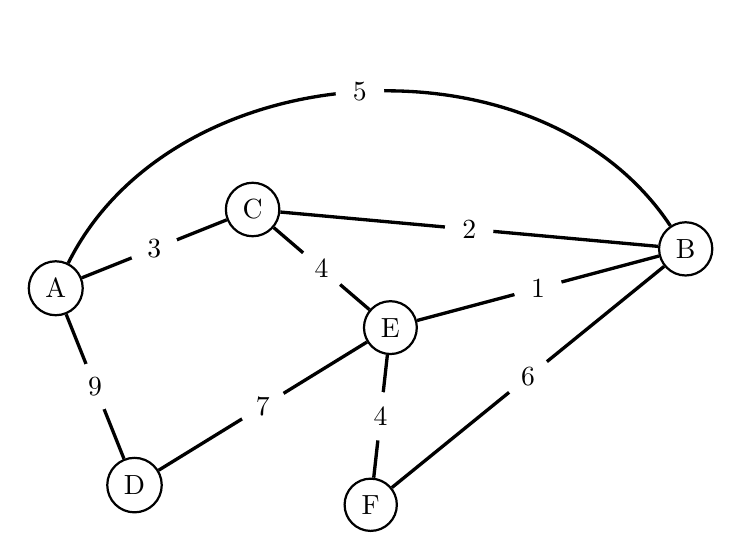
\begin{tikzpicture}
	\begin{scope}[every node/.style={circle,thick,draw}]
		\node (A) at (0,0) {A};
		\node (D) at (1,-2.5) {D};
		\node (F) at (4,-2.75) {F} ;
		\node (B) at (8,0.5) {B};
		\node (C) at (2.5,1) {C};
		\node (E) at (4.25,-0.5) {E};
	\end{scope}

	\begin{scope}[>={Stealth[black]},
		every node/.style={fill=white,circle},
		every edge/.style={draw=black,very thick}]
		\path (A) edge[bend left=60] node {$5$} (B);
		\path (A) edge node {$3$} (C);
		\path (A) edge node {$9$} (D);

		\path (B) edge node {$2$} (C);
		\path (B) edge node {$1$} (E);
		\path (B) edge node {$6$} (F);

		\path (C) edge node {$4$} (E);

		\path (D) edge node {$7$} (E);

		\path (E) edge node {$4$} (F);
	\end{scope}
\end{tikzpicture}
%\vspace*{0.5em}
%
%\begin{tikzpicture}
%	\begin{scope}[every node/.style={circle,thick,draw}]
%		\node (A) at (0,0) {A};
%		\node (B) at (0,3) {B};
%		\node (C) at (2.5,4) {C};
%		\node (D) at (2.5,1) {D};
%		\node (E) at (2.5,-3) {E};
%		\node (F) at (5,3) {F} ;
%	\end{scope}
%
%
%	\begin{scope}[>={Stealth[black]},
%		every node/.style={fill=white,circle},
%		every edge/.style={draw=red,very thick}]
%		\path [->] (A) edge node {$5$} (B);
%		\path [->] (B) edge node {$3$} (C);
%		\path [->] (A) edge node {$4$} (D);
%		\path [->] (D) edge node {$3$} (C);
%		\path [->] (A) edge node {$3$} (E);
%		\path [->] (D) edge node {$3$} (E);
%		\path [->] (D) edge node {$3$} (F);
%		\path [->] (C) edge node {$5$} (F);
%		\path [->] (E) edge node {$8$} (F);
%		\path [->] (B) edge[bend right=60] node {$1$} (E);
%	\end{scope}
%\end{tikzpicture}

\end{document}